\documentclass{article}
\usepackage{amsfonts, amsmath, amssymb, amsthm} % Math notations imported
\usepackage{enumitem}
\usepackage{graphicx}
\usepackage{setspace}
\usepackage{indentfirst}
\usepackage[margin=1in]{geometry}
\graphicspath{{./images/}} % Path to images

% \begin{figure}[htb!]
%      \centering
%      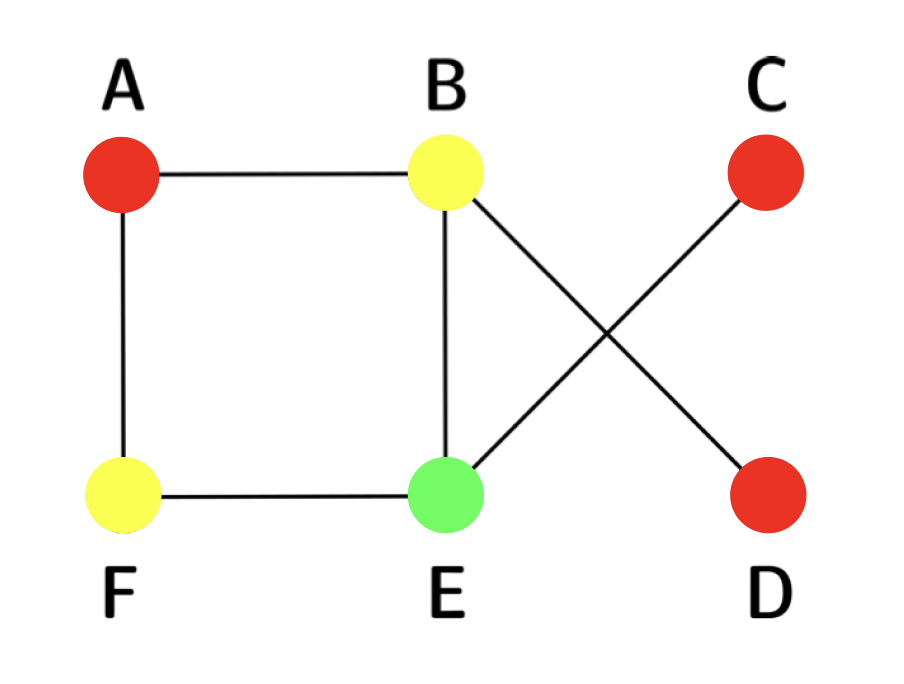
\includegraphics[scale=0.5]{coloring.png}
%      \caption{Coloring of the graph.}
% \end{figure}

% \begin{figure}[htb]
%     \qquad
%     \begin{minipage}{.4\textwidth}
%         \centering
%         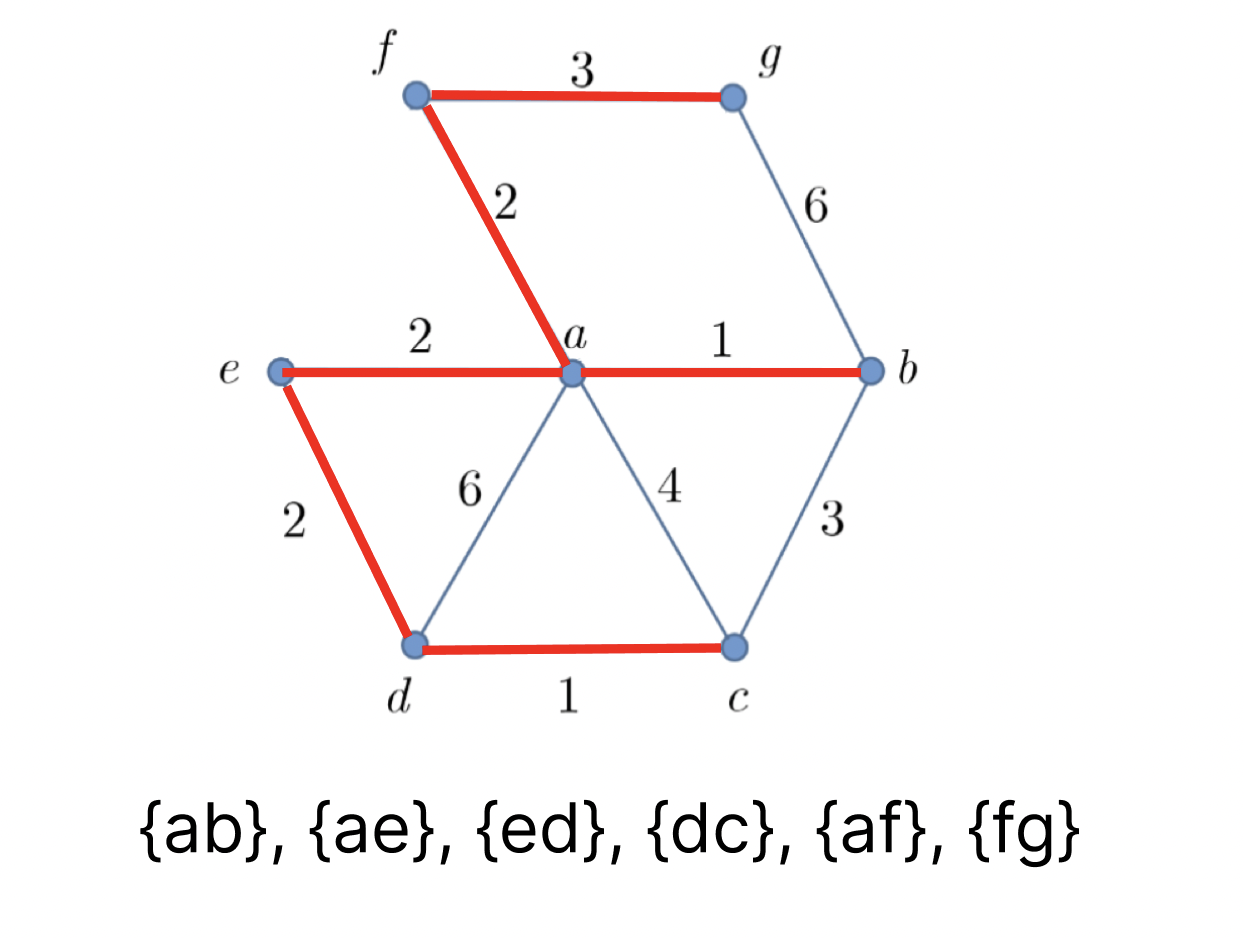
\includegraphics[scale=0.35]{prims.png}
%         \caption{}
%     \end{minipage}    
%     \qquad
%     \begin{minipage}{.4\textwidth}
%         \centering
%         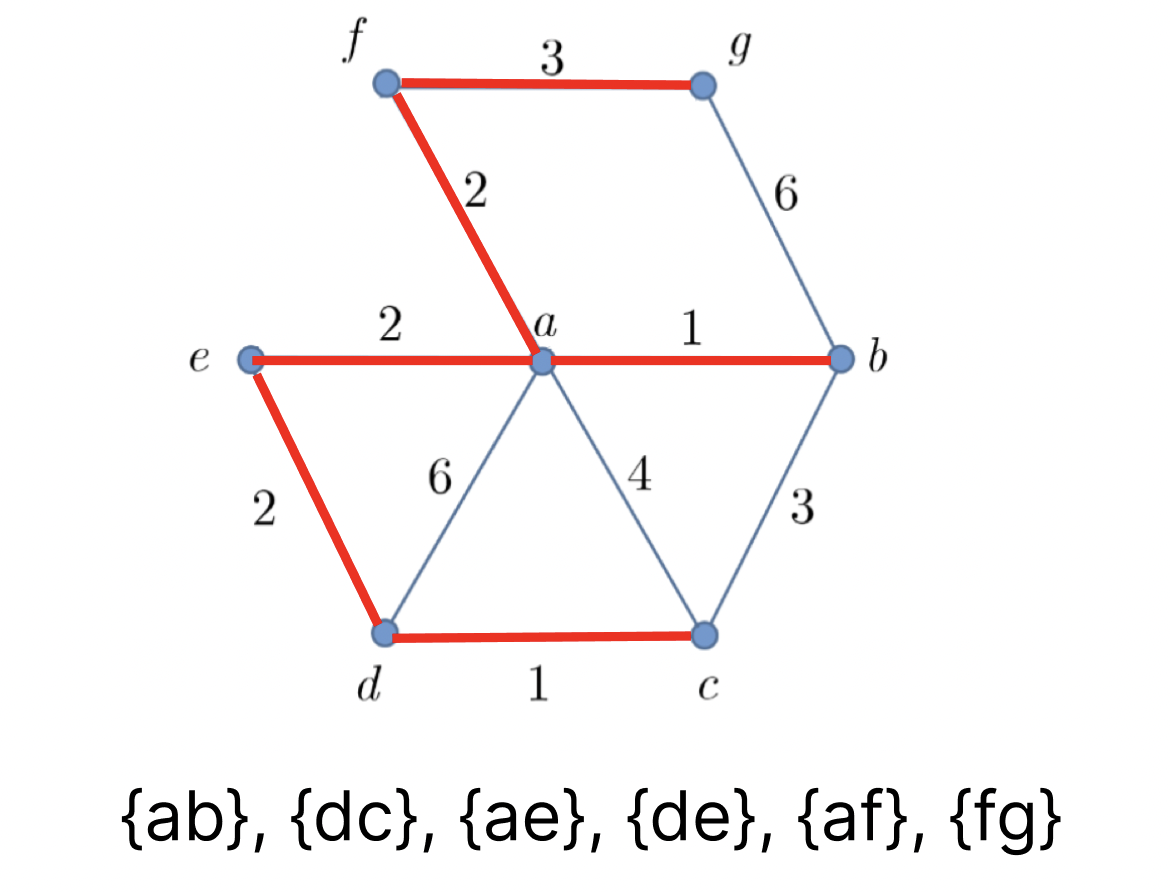
\includegraphics[scale=0.35]{kruskal.png}
%         \caption{}
%     \end{minipage}        
% \end{figure} 

\newtheorem{thm}{Theorem}
\newtheorem{proposition}[thm]{Proposition}
\newtheorem{cor}[thm]{Corollary}

% title information
\title{Math 104 HW3}
\author{Neo Lee}
\date{09/15/2023}

\setstretch{1.15}
% main content
\begin{document} 

% placing title information; comment out if using fancyhdr
\maketitle 
\section*{Exercise 7.4}
Give examples of 
\begin{enumerate}[label=(\alph*)]
    \item A sequence $(x_n)$ of irrational numbers having a limit $\lim x_n$ that is rational.
    \begin{proof}[Solution]
        Consider $(x_n) = \frac{1}{n}\cdot\sqrt{2}$. Clearly, $\lim x_n = 0$ and $x_n$ is 
        irrational for all $n$.
    \end{proof}
    \item A sequence $(r_n)$ of rational numbers having a limit $\lim x_n$ that is irrational.
    \begin{proof}[Solution]
        A simple one would be $(r_n) = 1 + \frac{1}{1!} + \frac{1}{2!} + \cdots + \frac{1}{n!}$.
        Certianly, $\lim r_n = e$ and $e$ is irrational, while $r_n$ is rational for all $n$.
    \end{proof}
\end{enumerate}

\section*{Exercise 7.5}
Determine the following limits. No proofs are required, but show any relevant algebra.
\begin{enumerate}[label=(\alph*)]
    \item $\lim s_n$ where $s_n=\sqrt{n^2+1}-n$. Hint: first show $s_n =\frac{1}{\sqrt{n^2+1}+n}$.
    \begin{proof}[Solution]
        \begin{align*}
            s_n & = \sqrt{n^2+1}-n \\
            & = \left(\sqrt{n^2+1}-n\right) \times \frac{\sqrt{n^2+1}+n}{\sqrt{n^2+1}+n} \\
            & = \frac{1}{\sqrt{n^2+1}+n} \\
            \lim s_n & = 0.
        \end{align*}
    \end{proof}
    \item $\lim (\sqrt{n^2+n}-n)$.
    \begin{proof}[Solution]
        \begin{align*}
            \sqrt{n^2+n}-n & = \frac{n}{\sqrt{n^2+n}+n} \\
            & = \frac{1}{\sqrt{1+\frac{1}{n}}+1} \\
            \lim \left(\sqrt{n^2+n}-n\right) & = \frac{1}{2}.
        \end{align*}
    \end{proof}
    \item $\lim (\sqrt{4n^2+n}-2n)$.
    \begin{proof}[Solution]
        \begin{align*}
            \sqrt{4n^2+n}-2n & = \frac{n}{\sqrt{4n^2+n}+2n} \\
            & = \frac{1}{\sqrt{4+\frac{1}{n}}+2} \\
            \lim \left(\sqrt{4n^2+n}-2n\right) & = \frac{1}{4}.
        \end{align*}
    \end{proof}
\end{enumerate}

\section*{Exercise 8.5}
\begin{enumerate}[label=(\alph*)]
    \item 
    \begin{proposition}
        Consider three sequences $(a_n)$, $(s_n)$, and $(c_n)$ such that $a_n \leq s_n \leq c_n$ 
        for all $n$ and $\lim a_n = \lim c_n = s$. Then, $\lim s_n = s$. This is called the 
        \textit{squeeze lemma}.
    \end{proposition}
    \begin{proof}
        For an arbitrary $\epsilon>0$, we know for $n > N_c$, $$|c_n-s|<\epsilon\Rightarrow 
        c_n<s+\epsilon$$ and for $m>N_a$, $$|a_m-s|<\epsilon\Rightarrow a_m>s-\epsilon.$$ 
        Now take for $N = \max\{N_c, N_a\}$, we have for $k>N$, $$s_k<c_k<s+
        \epsilon.$$ At the same time, $$s-\epsilon<a_k<s_k.$$ Hence, 
        $$s-\epsilon < s_k < s + \epsilon$$ and $|s_k-s| < \epsilon.$
    \end{proof}
    \item 
    \begin{proposition}
        Suppose $(s_n)$ and $(t_n)$ are sequences such that $|s_n| \leq t_n$ for all $n$ and 
        $\lim t_n = 0$. Then $\lim s_n = 0$.
    \end{proposition}
    \begin{proof}
        Notice $-t_n\le s_n\le t_n$. If we can show that $\lim (-t_n) = 0$, then by the squeeze 
        lemma, $\lim s_n = 0$. Now for an arbitrary $\epsilon>0$, take $n>N_t$, 
        $$|-t_n-0| = |t_n| = |t_n - 0|<\epsilon.$$ Hence, $\lim (-t_n) = 0$.
    \end{proof}
\end{enumerate}

\section*{Exercise 8.6}
Let $(s_n)$ be a sequence in $\mathbb{R}$.
\begin{enumerate}[label=(\alph*)]
    \item 
    \begin{proposition}
        $\lim s_n=0$ if and only if $\lim |s_n|=0$.
    \end{proposition}
    \begin{proof}
        For any $\epsilon>0$, we know $\exists N$ such that for $n>N$, 
        \begin{align*}
            |s_n-0| <\epsilon &\Leftrightarrow |s_n| < \epsilon \\
            &\Leftrightarrow |(|s_n|)| < \epsilon \\
            & \Leftrightarrow |(|s_n|)-0| < \epsilon.
        \end{align*}
    \end{proof}
\end{enumerate}

\section*{Exercise 8.9}
Let $(s_n)$ be a sequence that converges.
\begin{enumerate}[label=(\alph*)]
    \item 
    \begin{proposition}
        If $s_n\ge a$ for all but finitely many $n$, then $\lim s_n\ge a$.
    \end{proposition}
    \begin{proof}
        Assume for contradiction that $\lim s_n=s<a$, which 
        can be written as $a = s+2\epsilon$ for some $\epsilon>0$. Now take $N = max\{n:s_n<a\}$, 
        for all $n>N$, $$s_n \ge a = s+2\epsilon\Rightarrow |s_n-s|>\epsilon.$$

        This contradicts the definition of limit $\lim s_n = s$. Hence, $\lim s_n \ge a$.
    \end{proof}
    
    \item
    \begin{proposition}
        If $s_n\le b$ for all but finitely many $n$, then $\lim s_n \le b$.
    \end{proposition}
    \begin{proof}
        Similary, assume for contradiction that $\lim s_n=s>b$, which 
        can be written as $b = s-2\epsilon$ for some $\epsilon>0$. Now take $N = max\{n:s_n>b\}$, 
        for all $n>N$, $$s_n \le b = s-2\epsilon\Rightarrow |s_n-s|>\epsilon.$$
    
        This contradicts the definition of limit $\lim s_n = s$. Hence, $\lim s_n \le b$.
    \end{proof}

    \item
    \begin{proposition}
        If all but finitely many $s_n$ belong to $[a,b]$, then $\lim s_n$ belongs to $[a,b]$.
    \end{proposition}
    \begin{proof}
        It means for all but finitely many $n$, $s_n \le b$. Also, for all but finitely many $m$,
         and $s_m\ge a$. Following from (a) and 
        (b), then $\lim s_n \ge a$ and $\lim s_n \le b$. Hence $\lim s_n \in [a,b]$.
    \end{proof}
\end{enumerate}

\section*{Exercise 9.1a}
\begin{proposition}
    $\lim \frac{n+1}{n}=1$.
\end{proposition}
\begin{proof}
    \begin{align*}
        \lim \frac{n+1}{n} & = \lim \frac{1 + 1/n}{1} \\
        & = \lim (1+1/n) \cdot \lim 1 \\
        & = (\lim 1 + \lim 1/n)\cdot \lim 1 \\
        & = 1.
    \end{align*}
\end{proof}

\section*{Exercise 9.4}
Let $s_1=1$ and for $n\ge1$ let $s_{n+1}=\sqrt{s_n+1}$.
\begin{enumerate}[label=(\alph*)]
    \item List the first four terms of $(s_n)$.
    \begin{proof}[Solution]\indent
        \begin{enumerate}[label=\arabic*.]
            \item 1
            \item $\sqrt{2}$
            \item $\sqrt{\sqrt{2}+1}$
            \item $\sqrt{\sqrt{\sqrt{2}+1}+1}$
        \end{enumerate}
    \end{proof}

    \item
    \begin{proposition}
        Assume $(s_n)$ converges, then $\lim (s_n) = \frac{1}{2}\left(1+\sqrt{5}\right)$.
    \end{proposition}
    \begin{proof}
        Notice $\lim_{n\rightarrow\infty}s_{n+1} = s = \lim_{n\rightarrow\infty}s_n$. Hence, 
        \begin{align*}
            \lim_{n\rightarrow\infty} s_{n+1} & = \lim_{n\rightarrow\infty} \sqrt{s_n+1} \\
            \lim_{n\rightarrow\infty} s_{n+1} & = \sqrt{\lim_{n\rightarrow\infty} s_n+1} \\ 
            s & = \sqrt{s+1} \\
            s^2 - s - 1 & = 0.
        \end{align*}
        Solving the quadratic equation, we get $s = \frac{1}{2}\left(1\pm\sqrt{5}\right)$.
        Notice $s_n > 0$ for all $n$, so $\lim s_n\ge 0$ [check \emph{proposition 4}]. Thus, 
        $\lim (s_n) = \frac{1}{2}\left(1+\sqrt{5}\right)$.
        
        \newpage
        \emph{Attempt to prove $(s_n)$ converges:}

        We first show that $s_n$ is monotonic increasing in the interval 
        $I = \left(\frac{\left(1-\sqrt{5}\right)}{2}, \frac{\left(1+\sqrt{5}\right)}{2}\right)$. 
        Indeed, for $s_n\in I,$
        \begin{align*}
            s_n^2 - s_n - 1 & < 0 \\
            s_n^2 & < s_n + 1 \\
            s_n & < \sqrt{s_n + 1} \\
            s_n & < s_{n+1}.
        \end{align*}

        Then, we show that $(s_n)$ is bounded by $\frac{\left(1+\sqrt{5}\right)}{2}$. We proceed 
        with induction to show that $s_n < \frac{\left(1+\sqrt{5}\right)}{2}$ for all 
        $n\in\mathbb{N}$. The base case $s_1 = 1$ is trivial. Now assume 
        $s_k < \frac{\left(1+\sqrt{5}\right)}{2}$ for some $k\in\mathbb{N}$.
        To show $s_{k+1} < \frac{\left(1+\sqrt{5}\right)}{2}$, we need
        \begin{align*}
            \sqrt{s_k+1} & < \frac{\left(1+\sqrt{5}\right)}{2} \\ 
            s_k + 1 & < \frac{6 + 2\sqrt{5}}{4} \\
            s_k & < \frac{6 + 2\sqrt{5}}{4} - 1 \\ 
            s_k & < \frac{\left(1+\sqrt{5}\right)}{2},
        \end{align*}
        which is indeed true by our inductive hypothesis.

        Hence, by mathematical induction, $s_n = |s_n| < \frac{\left(1+\sqrt{5}\right)}{2}$ for all 
        $n\in\mathbb{N}$. Now, since $s_n$ is a bounded monotone, it converges.
    \end{proof}
\end{enumerate}

\end{document}
